\chapter{Appendix}
\section{Projects that have been already built upon Anacleto:}
\subsection{W7X - trigger }
\cite{RIGONI2018122}
The Anacleto framework has been used to develop a general purpose timing device to be used in Wendelstein 7-X diagnostics. The timing device is implemented in a Red Pitaya board and defines two digital outputs to generate clock and gate signals, and two digital inputs to receive a synchronizing 10 MHz clock and a trigger signal. The board is configured via software to generate a pre-programmed timing sequence after the system has been armed and a trigger input signal has been received. The timing sequence is communicated via TCP/IP to the ARM processor hosted in the Zynq chip of the Red Pitaya board. In this case a set of registers have been defined as interface between the processor and the FPGA application, without using interrupt lines. All registers except one are used to specify the time sequence. The remaining register is used as command register to arm and disarm the board. Not considering the time required for developing the FPGA application written in VHDL the creation of the new project, the adaption of the driver from the template and the deploy required less than one working day.

\begin{figure}
    \centering
    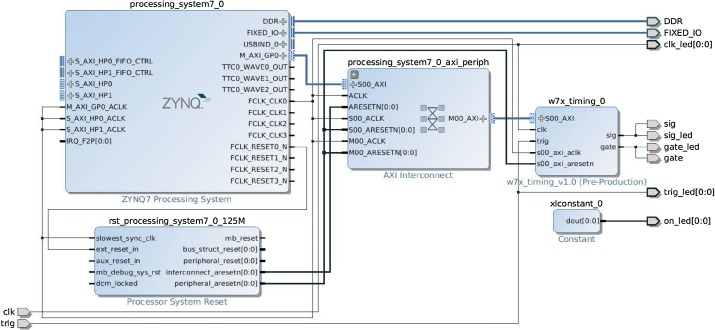
\includegraphics{img/APPENDIX/W7X_VHDL.jpg}
    \caption{W7X}
    \label{fig:W7X}
\end{figure}

\subsection{NIO fast daq}
%%
%% NIO ADC % ANDREA
%%
\section{fast event driven data acquisition for the NIO negative ion beam}
~

A desired topics for a DAQ device is the possibility to increase the level of detail during acquisition based on particular events. It is not uncommon to have an observed quantity that changes rapidly in time and than last steady or possibly in a non interesting state for long periods. An example of is the breakdown event that occurs in the accelerator grids of a ion source, leading to a very fast transient change in the measured currents and voltages of the grid power supply. In this case, fast data acquisition must be triggered by the event itself, acquiring data for a short time window around the event occurrence. This technique has been applied to Nio experiment~\cite{DEMURI2015249} a small radio frequency negative ions beam source with a high voltage electrostatic particle accelerator stage composed of grids. In certain conditions break-down events~\cite{RECCHIA20111545} appear on the high voltage gaps of the grids causing a  high current discharges of the power supply feeding the accelerator. 
~
A subset of the FPGA functionality described in section 3 has been implemented in a Red Pitaya device, namely the trigger logic to detect the occurrence of the event, the pre and post trigger sampling logic and the FIFO/DMA data transfer to computer memory via the GNU Linux driver. In this case data are streamed and when an event is detected and data collected at 5 MHz sampling speed along the corresponding time window, the data block is passed, either via FIFO or DMA, to the linux driver and then, in turn, to a program in the Zynq processor that communicates the newly acquired data block to the central data acquisition system via TCP/IP. The results are displayed in Fig. 4, showing the events acquired during a beam generation lasting 2 hours. Each time window lasts 1 ms, and one enlarged event is  displayed in the lower part of Fig. 4.    
\begin{figure}
\centering
%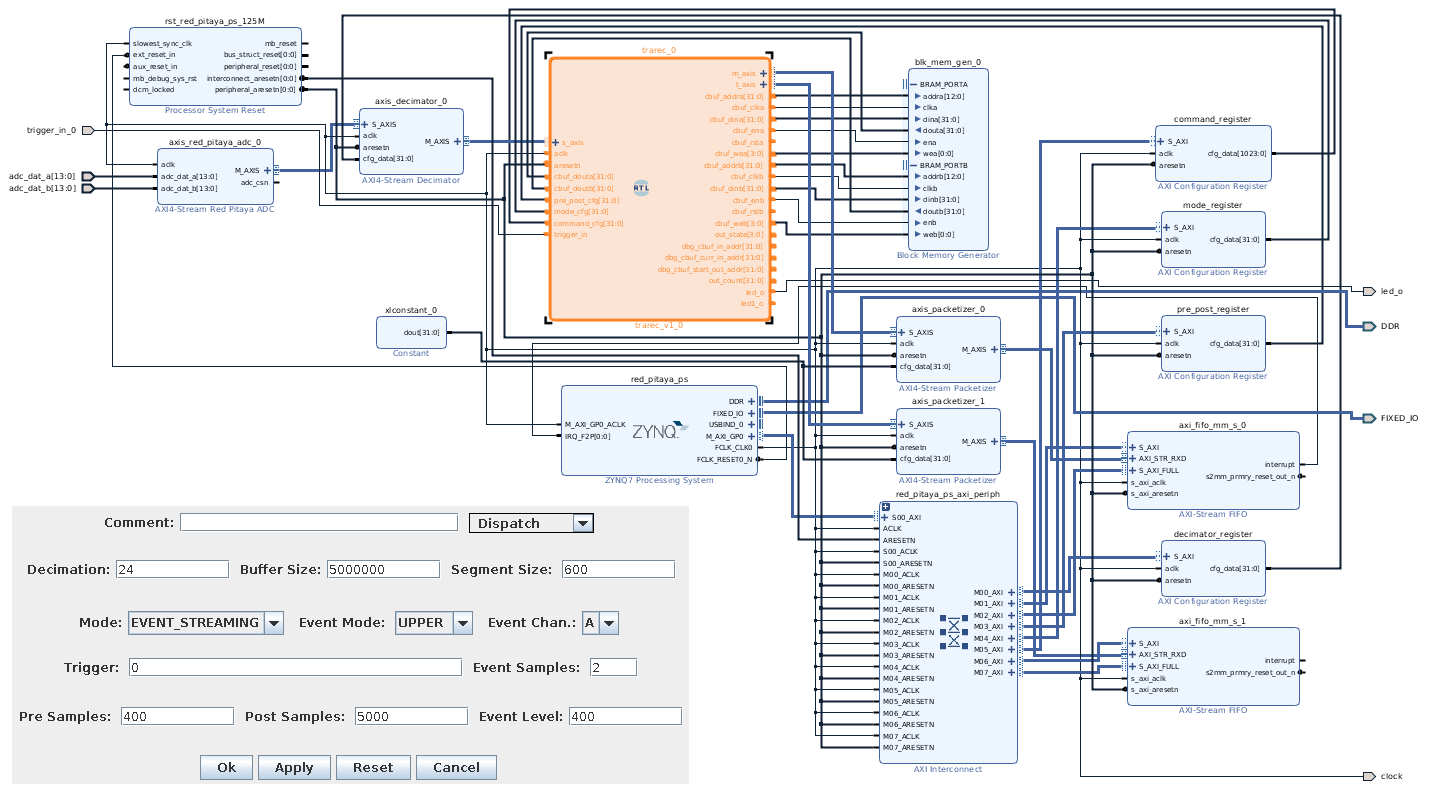
\includegraphics[width=0.59\textwidth]{img/nio_scm1.png}
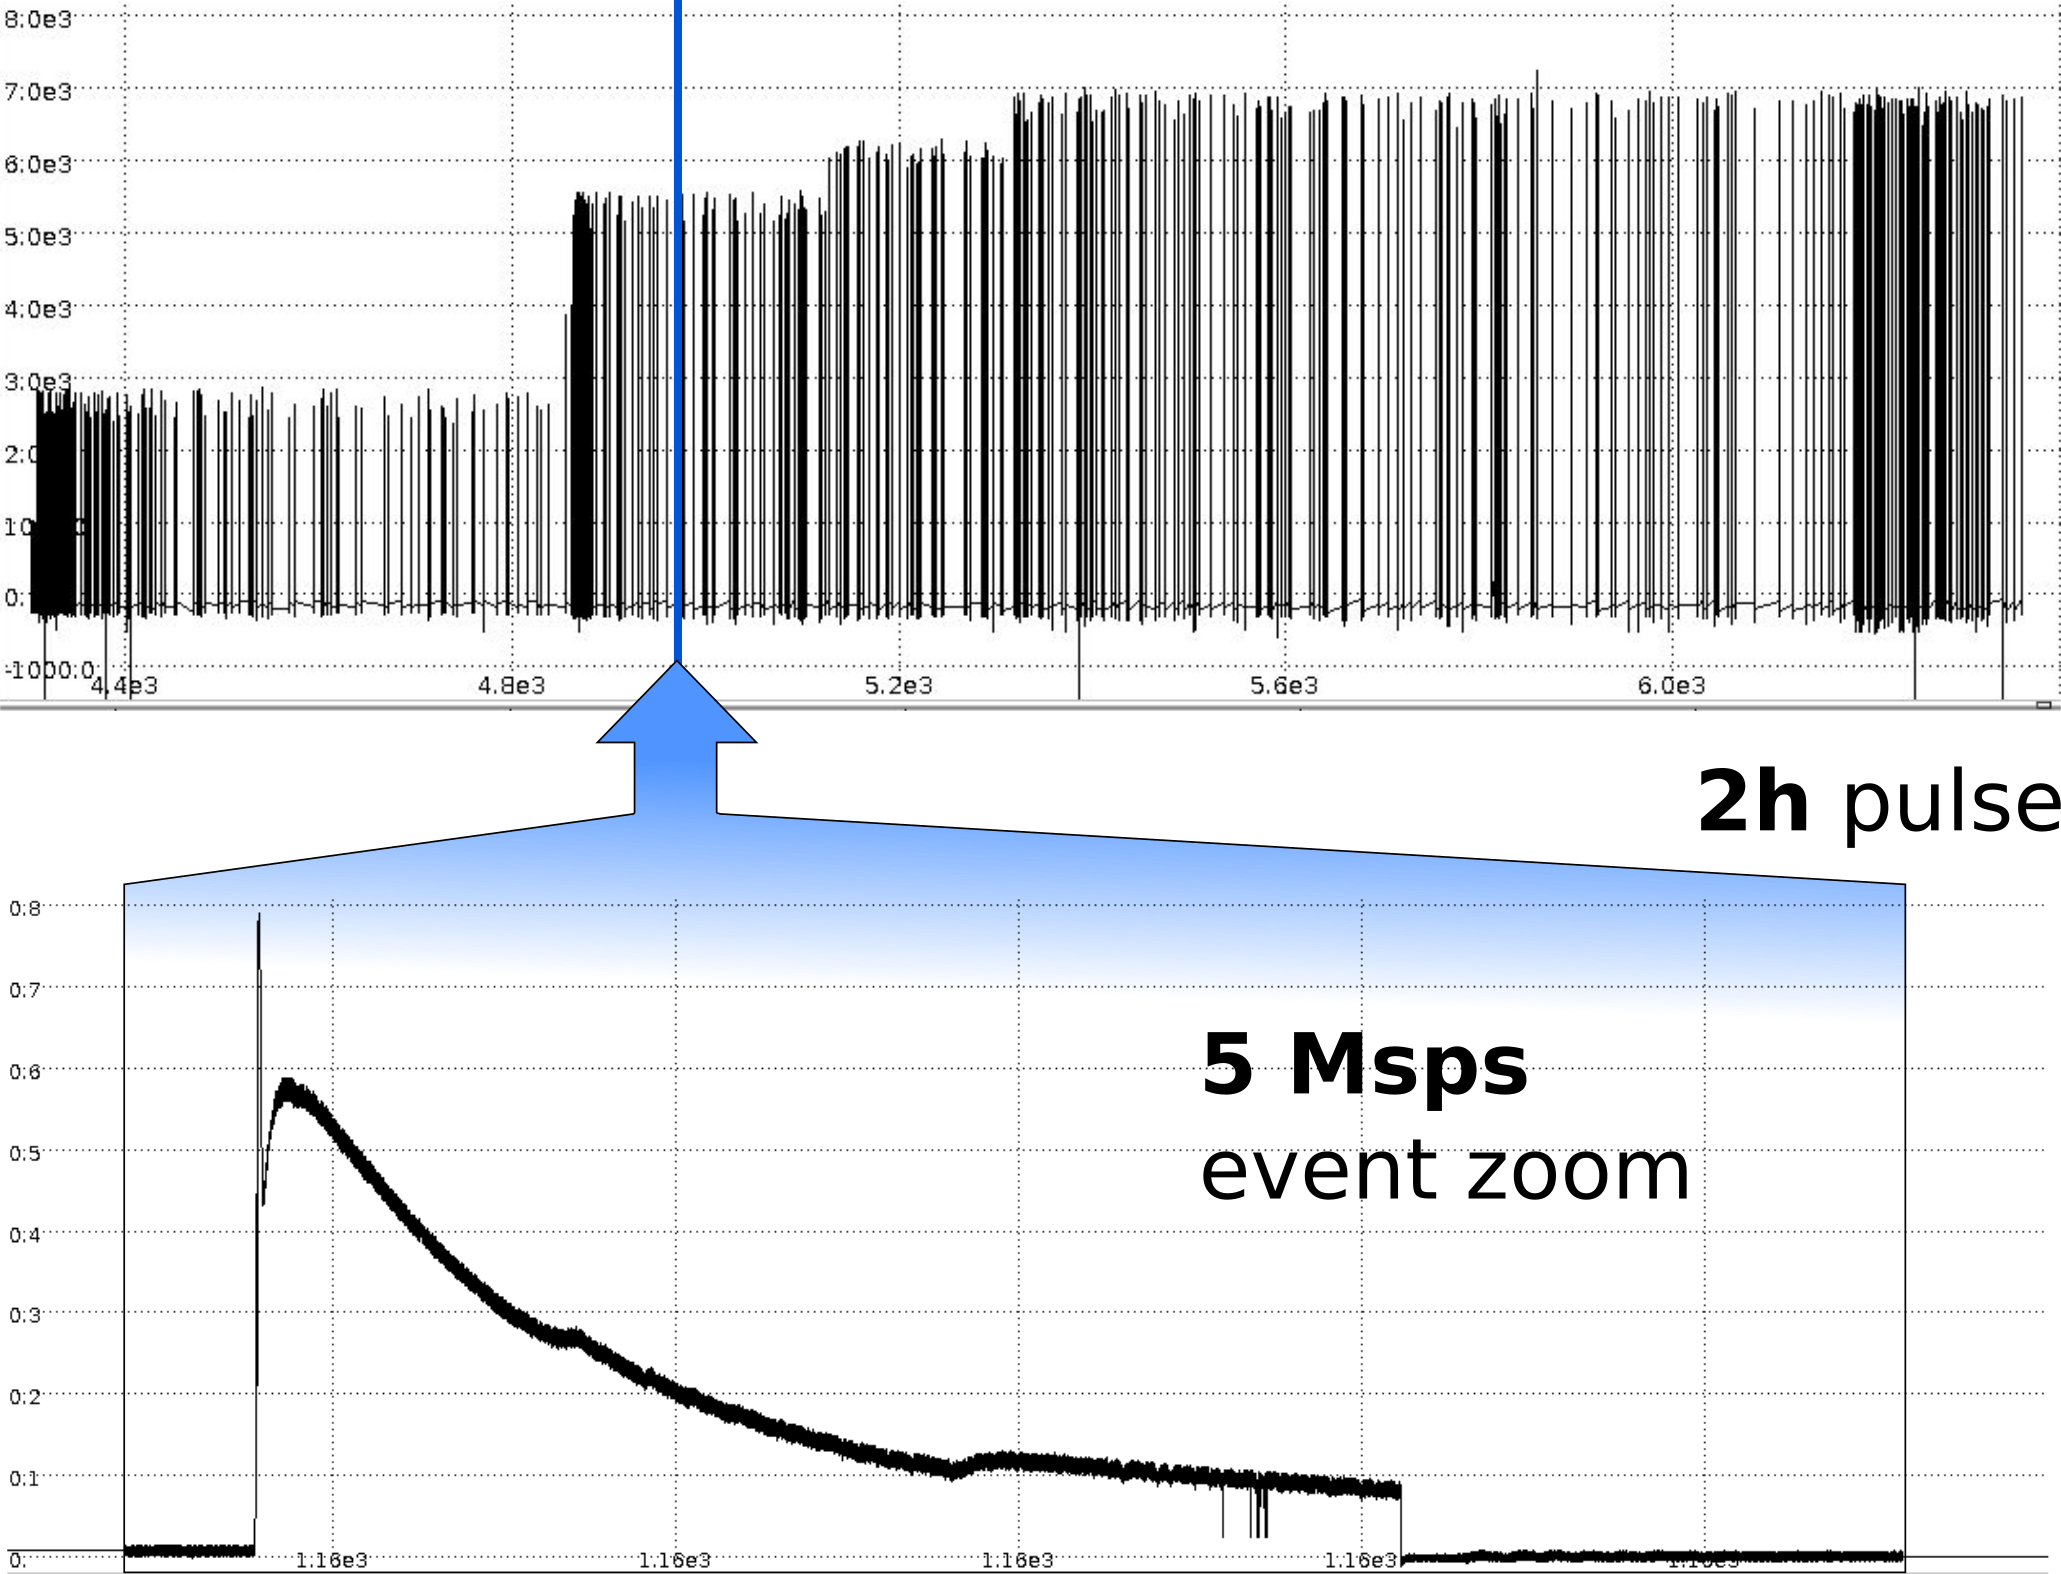
\includegraphics[width=0.49\textwidth]{img/4_EmbeddedML/nio12b.png}
\caption{figure example.}
\label{fig:nio}
\end{figure}


\subsection{Spider Redpitaya}

\section{Projects that have been already built upon Tensorflow:}

\subsection{Jasper and Horace }
